
\documentclass{standalone}
\usepackage{xcolor}
\usepackage{pgfplots}
\pgfplotsset{compat=1.18}

\begin{document}

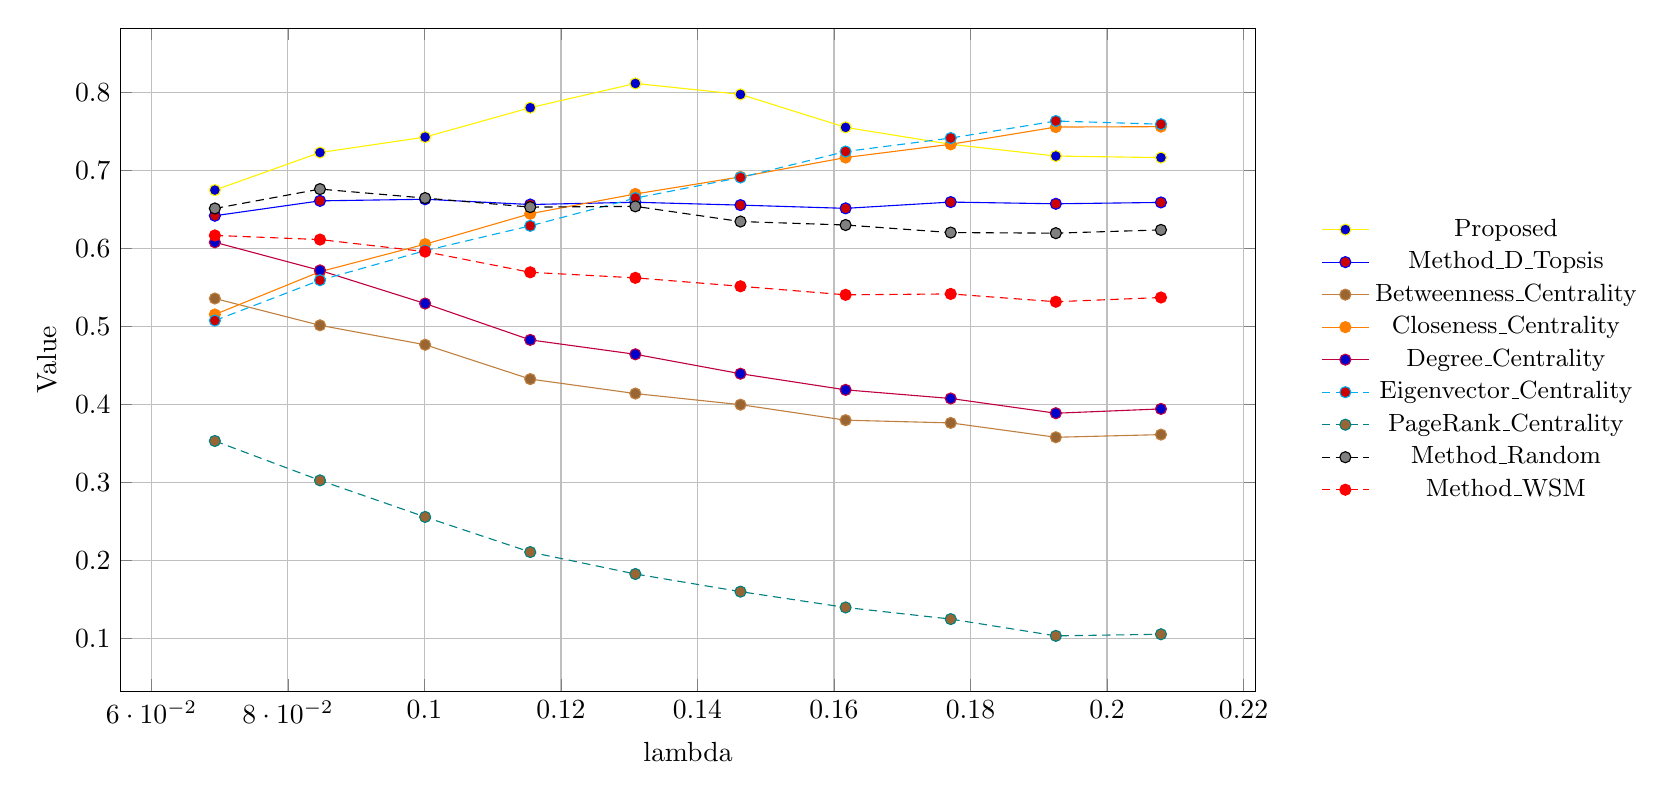
\begin{tikzpicture}
\begin{axis}[
    width=16cm,
    height=10cm,
    xlabel={lambda},
    ylabel={Value},
    grid=major,
    legend style={
        at={(1.05,0.5)},
        anchor=west,
        font=\small,
        draw=none,
        cells={align=left},
    },
]
% Proposed
\addplot+[color=yellow, mark=*] coordinates {
(0.0693,0.6749945715261746) (0.0847,0.7231452133524391) (0.1001,0.7429863889381317) (0.1155,0.7807235591417093) (0.1309,0.8117744319139951) (0.1463,0.7977555388063025) (0.1617,0.7554693952810599) (0.1771,0.733749025080185) (0.1925,0.7186662741321377) (0.2079,0.7166382065369119) };
\addlegendentry{Proposed}

% Method\_D\_Topsis
\addplot+[color=blue, mark=*] coordinates {
(0.0693,0.6420961179765284) (0.0847,0.6611850343867327) (0.1001,0.6632246974447704) (0.1155,0.656475944992773) (0.1309,0.6593895947836432) (0.1463,0.6557148117631936) (0.1617,0.6515749439390556) (0.1771,0.6596157992368328) (0.1925,0.6574097181438855) (0.2079,0.6591602424635313) };
\addlegendentry{Method\_D\_Topsis}

% Betweenness\_Centrality
\addplot+[color=brown, mark=*] coordinates {
(0.0693,0.5359118173019006) (0.0847,0.5015153010015241) (0.1001,0.4765954513768378) (0.1155,0.4325388315273679) (0.1309,0.413965475851972) (0.1463,0.3997138003034647) (0.1617,0.3798274786094618) (0.1771,0.3763143115837695) (0.1925,0.3578997280411134) (0.2079,0.3613075373132878) };
\addlegendentry{Betweenness\_Centrality}

% Closeness\_Centrality
\addplot+[color=orange, mark=*] coordinates {
(0.0693,0.5154199363221195) (0.0847,0.5702797470854958) (0.1001,0.6055976204241724) (0.1155,0.6446671927783663) (0.1309,0.6700225625360736) (0.1463,0.6919017980544908) (0.1617,0.7167424063700718) (0.1771,0.7337527321309736) (0.1925,0.755855073447505) (0.2079,0.756375066706915) };
\addlegendentry{Closeness\_Centrality}

% Degree\_Centrality
\addplot+[color=purple, mark=*] coordinates {
(0.0693,0.6080408823382267) (0.0847,0.5719705234429956) (0.1001,0.5294643589695628) (0.1155,0.4828276198626529) (0.1309,0.4643376765114954) (0.1463,0.4394316889627033) (0.1617,0.4187279244066215) (0.1771,0.4076478686557832) (0.1925,0.3887509277430958) (0.2079,0.3942712045377495) };
\addlegendentry{Degree\_Centrality}

% Eigenvector\_Centrality
\addplot+[color=cyan, mark=*] coordinates {
(0.0693,0.5076204975067753) (0.0847,0.5593712821922675) (0.1001,0.597271779685311) (0.1155,0.6291143638225875) (0.1309,0.6647190133628043) (0.1463,0.691169265134168) (0.1617,0.7244697795733027) (0.1771,0.741739370050448) (0.1925,0.7635937681330747) (0.2079,0.7595199729624338) };
\addlegendentry{Eigenvector\_Centrality}

% PageRank\_Centrality
\addplot+[color=teal, mark=*] coordinates {
(0.0693,0.3531380922354895) (0.0847,0.3026168921572899) (0.1001,0.2556890297220155) (0.1155,0.2106405105595595) (0.1309,0.1824877444948625) (0.1463,0.1598673931121148) (0.1617,0.1396021897115814) (0.1771,0.1246799488975271) (0.1925,0.1031326678686791) (0.2079,0.1052163500842298) };
\addlegendentry{PageRank\_Centrality}

% Method\_Random
\addplot+[color=black, mark=*] coordinates {
(0.0693,0.6514124786032774) (0.0847,0.6762681748903162) (0.1001,0.6647539081777342) (0.1155,0.6531613654610637) (0.1309,0.6541206137128868) (0.1463,0.6346557937769991) (0.1617,0.6301906042525316) (0.1771,0.620503111615294) (0.1925,0.6197347420722642) (0.2079,0.6239068406765642) };
\addlegendentry{Method\_Random}

% Method\_WSM
\addplot+[color=red, mark=*] coordinates {
(0.0693,0.6168380697806694) (0.0847,0.6115151809305328) (0.1001,0.5960484336703449) (0.1155,0.569515180135972) (0.1309,0.5624262535201371) (0.1463,0.5515840931783077) (0.1617,0.5406138448281037) (0.1771,0.5417838218612238) (0.1925,0.5317717552088757) (0.2079,0.5371878325164482) };
\addlegendentry{Method\_WSM}


\end{axis}
\end{tikzpicture}

\end{document}
